\section{Sparse Matrices and Solid Boolean Algebras}\label{boolean-algebras}
%=================================================

Manuscript~\cite{paoluzzi2019finite} shows that the set of join-irreducible atoms of the Boolean Algebra generated by a partition of $\E^3$ are one-to-one with the basis of 3-chain space also generated by the partition, and hence with the columns of the $[\partial_3]$ matrix, which provides a boundary representation (as 2-cycles) of the independent elements of 3-space. 
An example of such space decomposition is shown in Figures~\ref{fig:image1} and~\ref{fig:image2}. The 3-cells are not in scale, and are suitably rotated to better exhibit their
complex structure, even containing internal holes. Their assembly gives the union of the five cubes. Each
\emph{3-cell is generated} as \emph{a column} of the \emph{sparse matrix} of
\emph{chain map} $\partial_3: C_3\to C_2$,  with values in $\{-1,0,1\}$.
They are the join-irreducible \emph{atoms} of the CSG algebra with closed regular cells.

\begin{figure}[htbp]
    \centering
    \begin{minipage}{0.475\textwidth}
        \centering
       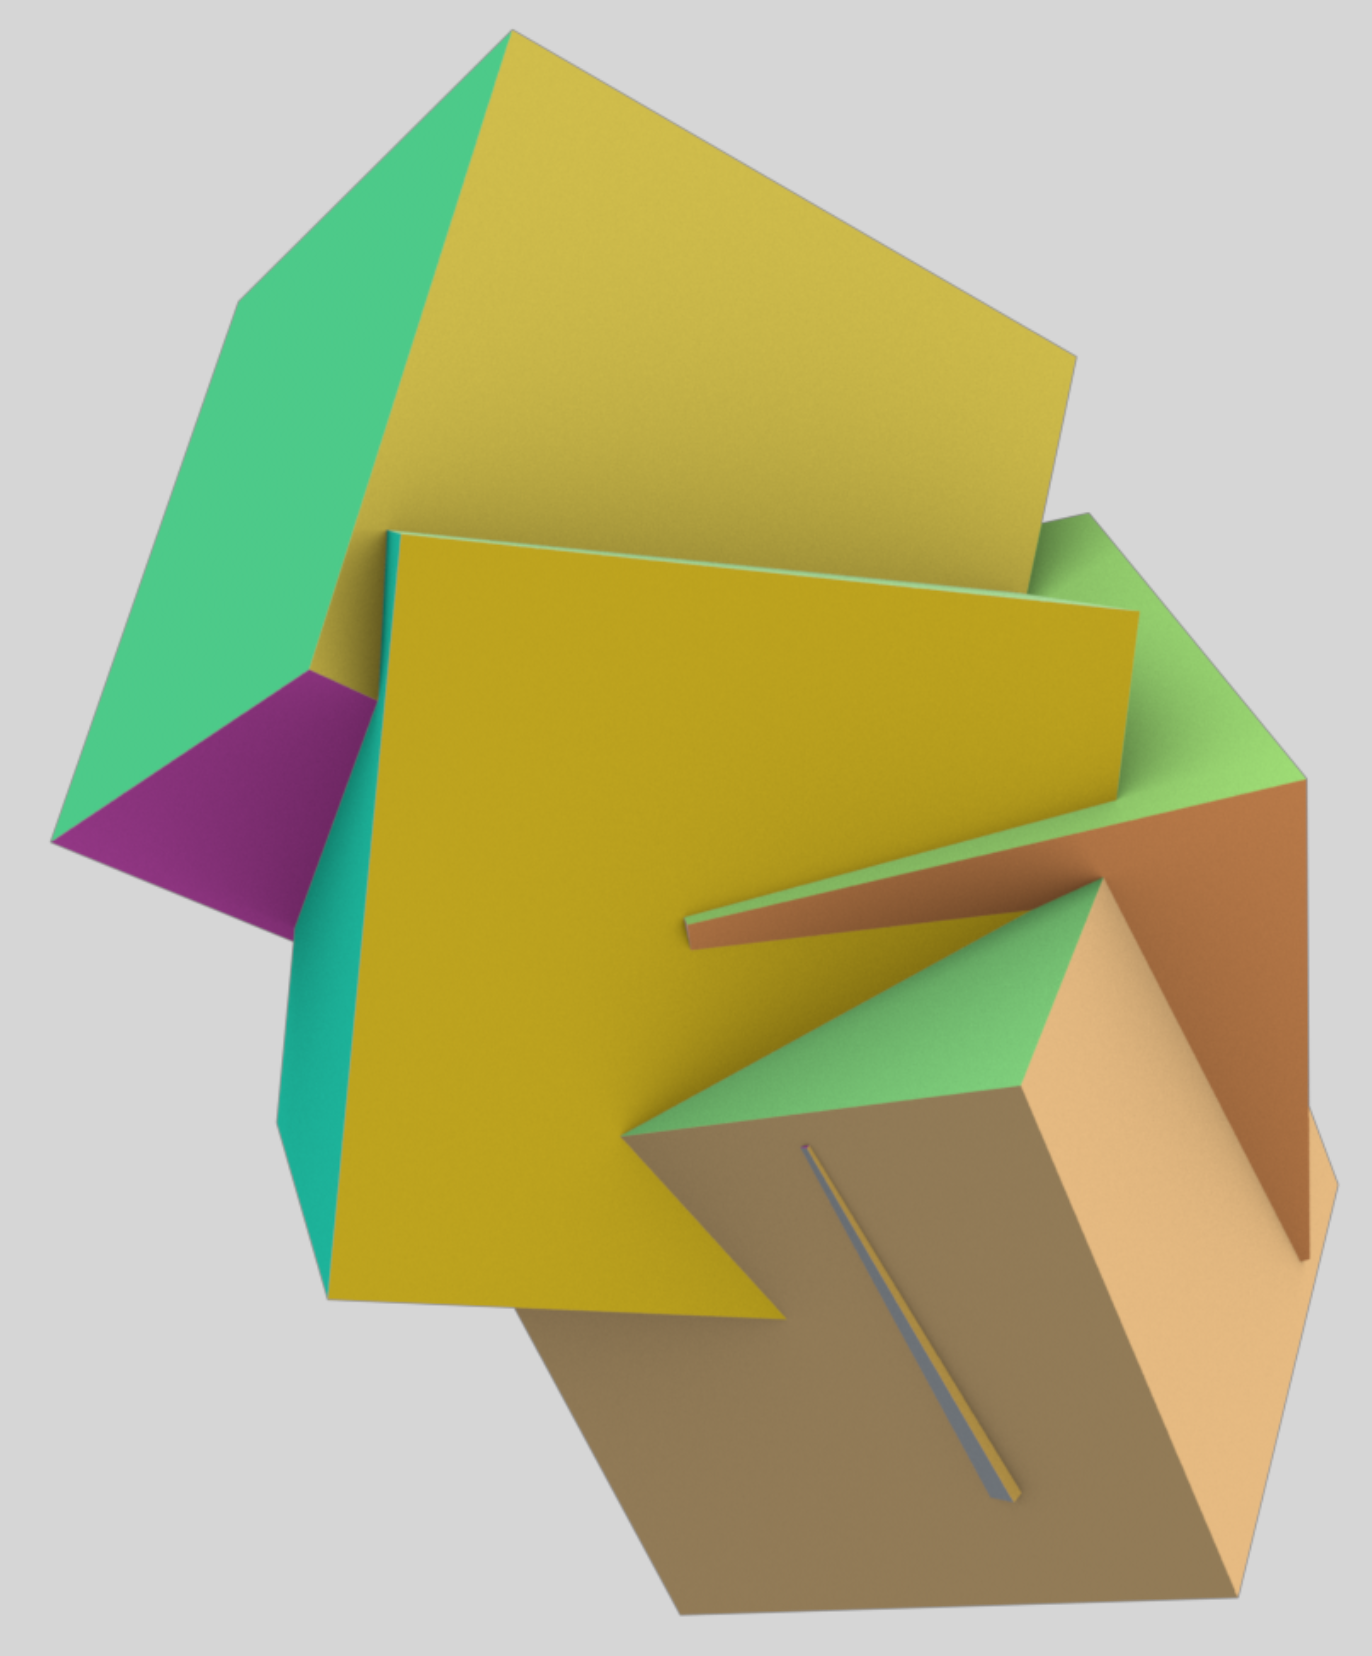
\includegraphics[width=0.6\linewidth]{../figs/image1.png} 
       \caption{A collection $\mathcal{S}$ of five random cubes in 3D Euclidean space.}
       \label{fig:image1}
    \end{minipage}\hfill
    \begin{minipage}{0.475\textwidth}
        \centering
       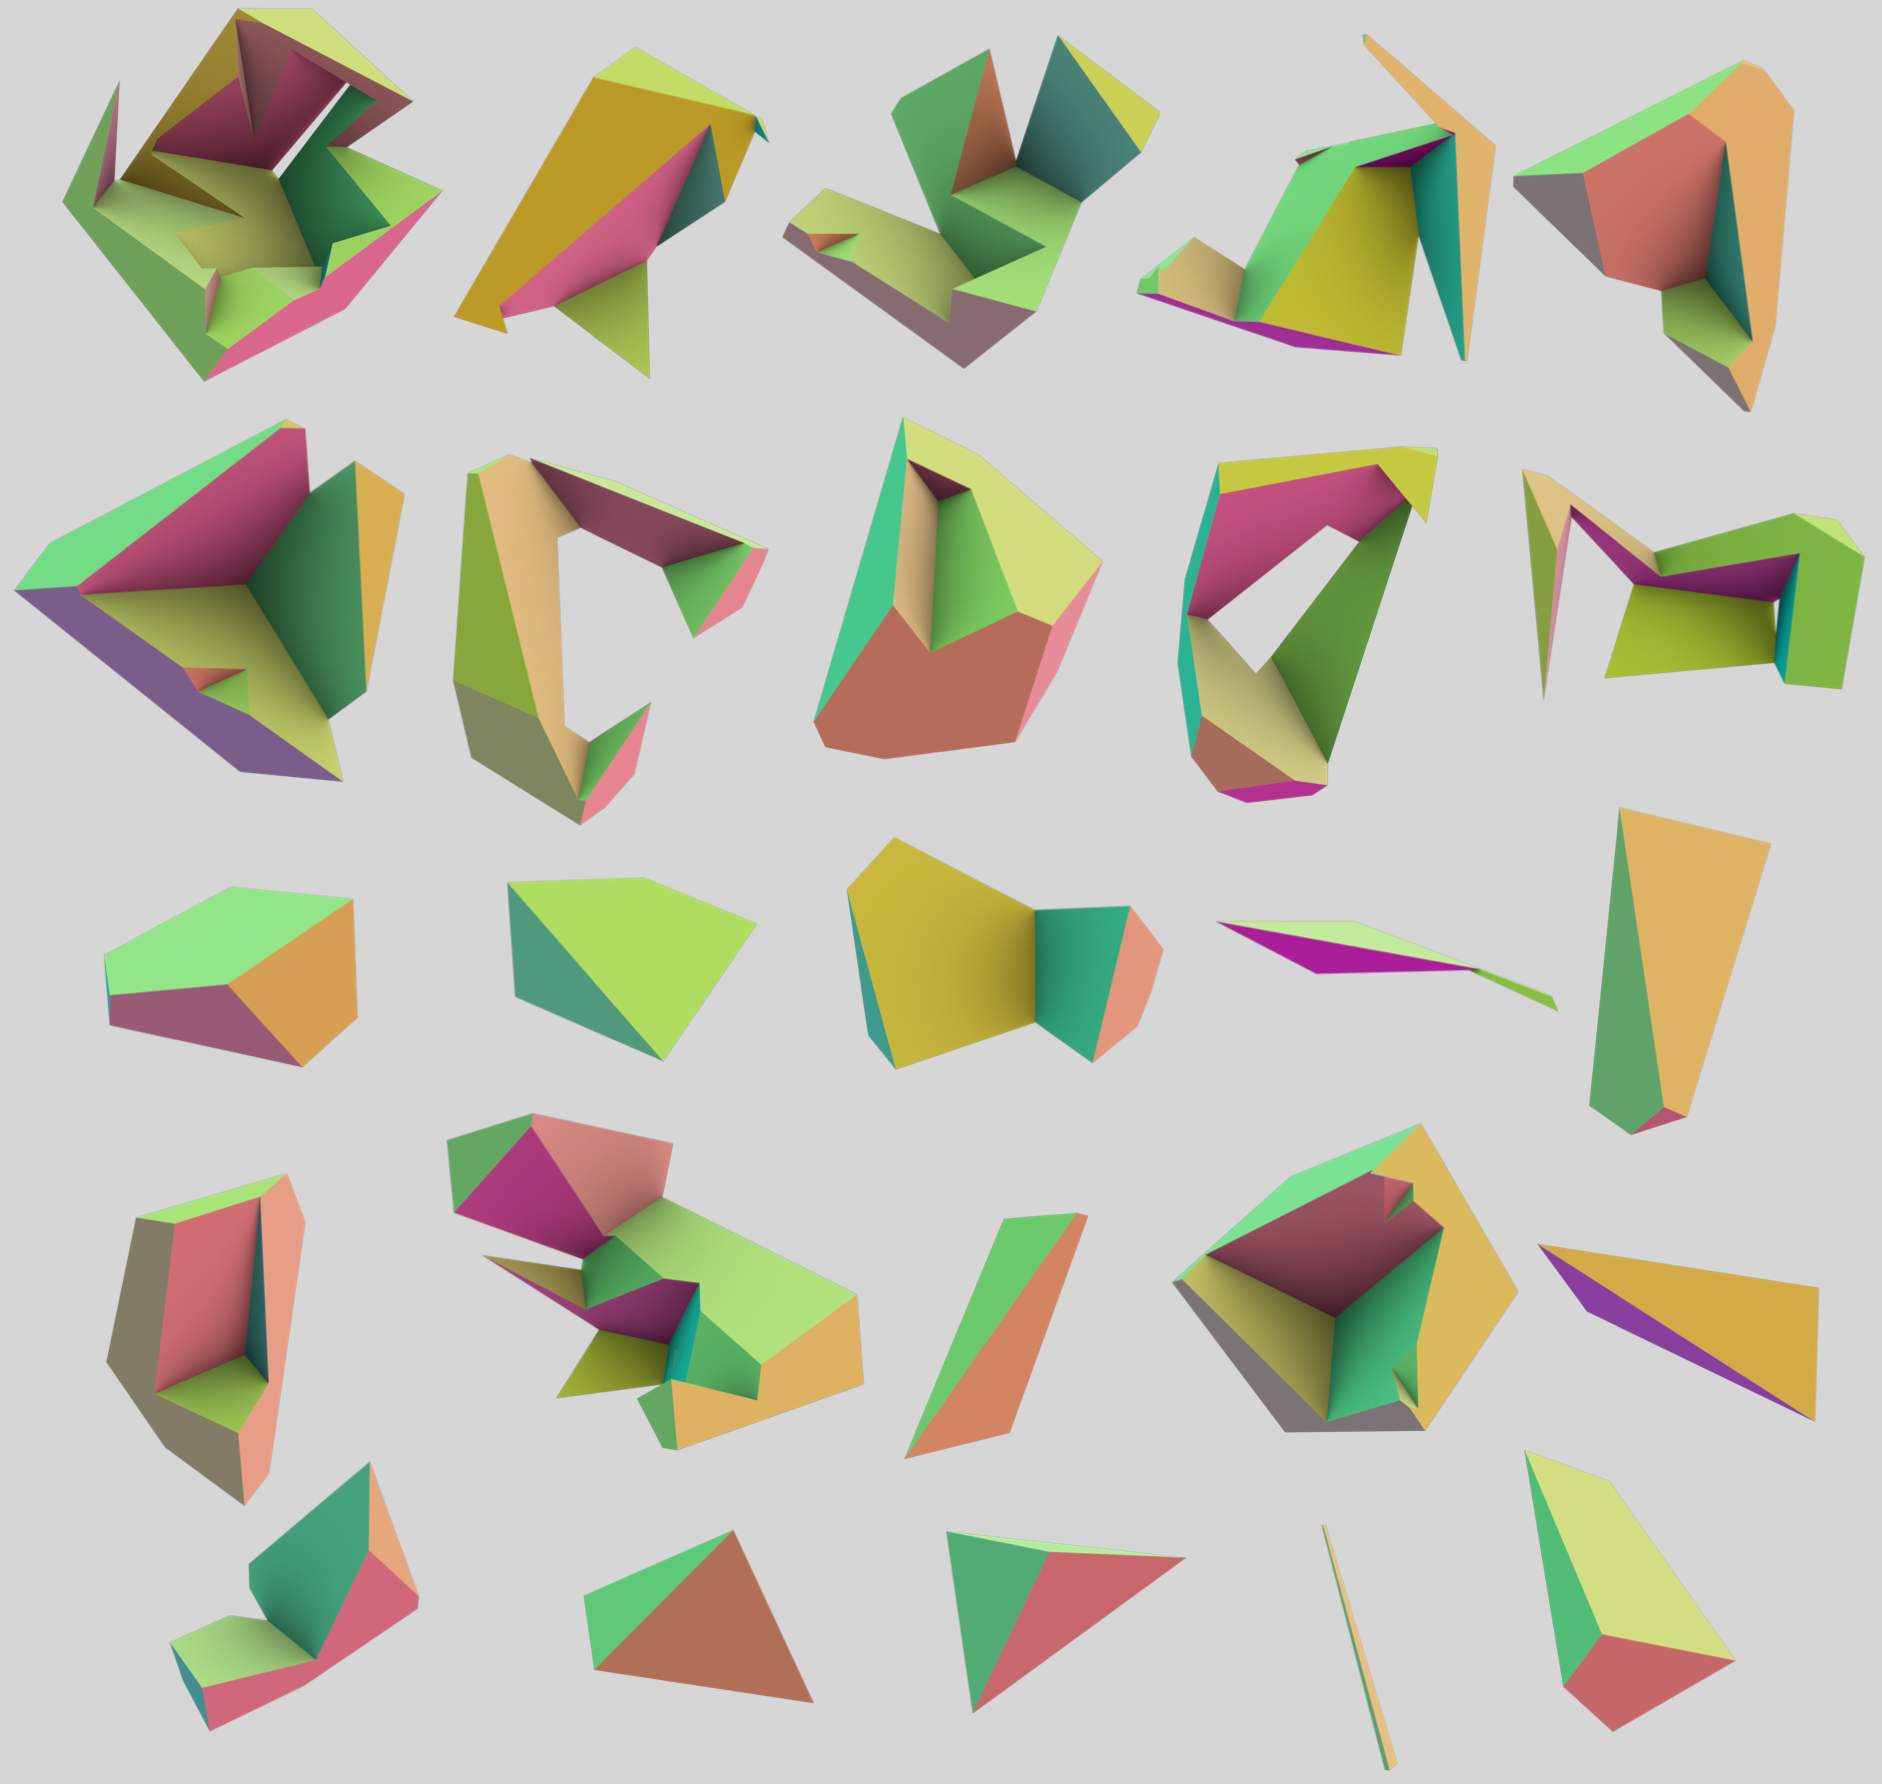
\includegraphics[width=0.8\linewidth]{../figs/image2.png} 
        \caption{3-cells of the generated arrangement $\mathcal{A}(\mathcal{S})$ of $\E^3$.
        They are given by columns of $[\partial_3]$ as \emph{atoms} of a solid Boolean algebra.}
       \label{fig:image2}
    \end{minipage}
\end{figure}

To generate the $d$-space arrangement induced by a collection of cellular ($d$--1)-complexes, some numerical algebra and basic tools of linear algebra and algebraic topology are used. In particular, (sparse) matrices of operators and matrix multiplication and transposition. Interval-trees and $kd$-trees are also introduced for acceleration of clustering of face cells into subsets of congruent shape. 

Using our approach with sparse matrices, the validity of topological computations is guaranteed, since these operator matrices must satisfy by construction the (graded) constraints: $[\partial_2][\partial_3]=[0]$ and $[\partial_1][\partial_2]=[0]$.  Similarly, we have $[\delta_1][\delta_0]=[0]$ and $[\delta_2][\delta_1]=[0]$.

With our approach based on boundary operators, the distinctions are removed between manifold and non-manifold representations (fairly standard in Solid Modeling), so allowing for mixing B-reps, cellular decompositions of elementary solids, and/or regular grids. This allows, e.g., for the generation of internal structures and mixed-dimensional objects needed in many applications, for example to make stronger and more resilient the ones to be produced via 3D printing.

Even more, the evaluation of CSG expressions of arbitrary complexity is done in a novel way, by combining the binary columns of 3D basis elements (i.e., the elements of the $U_3$ basis) with native Julia's operators for bitwise operations. In other words, once the $3$-space partition is generated, and $3$-cells are classified w.r.t.~all solids terms, via a single point-set containment test,  \emph{all CSG algebraic  expressions}---of any complexity---can be  evaluated simply by bitwise vectorized logical operations. 
Finally, the sparse matrix approach can be extended to general dimensions and/or implemented on highly parallel computational engines, even using standard GPU computing kernels.


